\section*{Problem No.3} \label{sec:prob3}
\paragraph{Part A:}
We construct a very simple mathematical model in order to solve the problem optimally. The model takes as input the edge list $E$. We have one decision variable $X \in \{0,1\}$ such that $X_{i}=1$ if vertex $i \in S$. The model then tries to directly maximize the number of vertices being influenced by maximizing the \emph{sum} of vertices that are being influenced $N(S)$. Concretely, the model can be written as 

\[
\begin{array}{cl}
\text{maximize} &  \sum_{i=1}^{n} max\left( X_{i}, \max_{(i,j)\in E}X_j \right)\\
\text{subject to} & |X|_{1} \leq K
\end{array} 
\]

Note that we choose to take the $max$ since if we computed the $sum$ instead, the computation won't reflect the problem correctly. This is because if a vertex $i$ is connected to two vertices $j$ and $k$ such that $j \in S$ and $k \in S$, the sum will return 2 while we want it to return 1. However, we would expect that $i$ returns just 1. 


Even thought the model is really simple and straightforward, we could not execute it using SCIP and ZIMPL modeling language. This is primarily because ZIMPL does not allow $max$ in the objective function. Another direction that we tried is to use an $if$ statement. The model can be written as:
\mathleft
\[
\mathtt{maximize\ myObjFunc:\ sum <V>\ in\ vertSet: } 
\]
\[
\qquad \qquad \qquad \qquad \qquad \mathtt{if\ (sum\ <V,j>\ in\ M:\ X[j]\ >=\ 0)\ then\ 1}
\]
\[
\qquad \qquad \qquad \qquad \qquad \mathtt{else\ 0\ end;}
\]

However, this model won't run because SCIP does not allow if statement in the objective function. To allow the model to run, we had to write it in away that only have $sum$ expressions. The trick we used here is to express $max$ and $min$ using the Quadratic Formula. The quadratic formula defines $max(a,b)= \frac{1}{2}\left(a+b + |a-b| \right)$ and $min(a,b)= \frac{1}{2}\left(a+b - |a-b| \right)$. This formula only computes the $max$ or $min$ between two numbers. We can recognize that the  (deep) inner $sum$ in the objective function we defined at the beginning can be simply re-written as $min$ of two numbers as follows
$$
\max_{(i,j)\in E}X_j = \min(\sum_{(i,j)\in E} X_j ,1)
$$
In other words, if the vertex $i$ is not connected to any vertex that is in $S$, then this $min$ will return 0 (min(0,1)). If vertex $i$ is connected to one or more vertex that is in $S$, the $min$ function will return 1. Since the $min$ is between two numbers, we can use the Quadratic Formula and implement it using SCIP. The only thing left is to consider that $N(S)$ also include the vertices in $S$ (the outer $max$ in the objective function). Since this $max$ is between two number, we can use the Quadratic Formula again. Finally, our objective function is expressed as
\mathcenter
\[
\begin{array}{cl}
\text{maximize} &  \sum_{i=1}^{n} \max \left\lbrace  \min\left\lbrace   \sum_{(i,j)\in E}X_j ,1 \right\rbrace,  X_{i}\right\rbrace\\
\text{subject to} & |X|_{1} \leq K
\end{array} 
\]

where the $max$ and $min$ are written as in the Quadratic Formula. We implemented this model using SCIP. We had to pre-process the input graph such that and edge between $i$ and $j$ is written twice; one time as $i$ the first vertex and second time as $j$. We also had to make sure that indexing starts with 1 (not 0). The model was tested it over small graph with 20 and 30 vertices with different values of $K$. At all cases, the model returns the optimal values correctly. However, we run the model using the facebook which has 4039 vertex and $K=1$ (for which we know the optimal solution), the model keep running for a long time (~ 3 hours) without giving an answer. 

%Here is our ZIMPL script 
%\begin{lstlisting}
%#Number of vertices in the graph, size of S
%param N := 4039;

%#The size of set S 
%set vertSet := {1 .. N}; 

%#The decision variable  
%var X[vertSet] binary;

%#Read the graph edges into matrix M
%set M:= {read "facebookgraph.txt" as "<1n, 2n>"};

%#Define the constraints 
%subto X_norm: sum<i> in vertSet : X[i] <= K;

%#Define objective func 
%maximize myObjFunc: sum <V> in vertSet : max <V,j> in M: X[j];
%\end{lstlisting}

%Another attempt we tried was to redefine the objective function using and $if$ statement as follows
%\begin{lstlisting}
%maximize myObjFunc: sum <V> in vertSet : 				
%				       if (sum <V,j> in M: X[j] >= 0) then 1 
%					   else 0 end;
%\end{lstlisting}

%This solution basically add one to the summation equation if the vertex is connected to at least one vertex in $S$, otherwise it adds zero. However, ZIMPL does not allow $if$ statements that uses the decision variables in the objective function. 

%For that, we decided to use MATLAB's $\mathtt{ga}$ function that tries to fine the minimum of objective function using genetic algorithm. Since $\mathtt{ga}$ only solves minimization, we change the objective function by multiplying it by -1. The code is attached and it requires Global Optimization Toolbox to run. The code has been tests on small graphs of 20 nodes with different $K$ values and it always produces the optimal values. However, with the Facebook graph, the \begin{large}TO DO\end{large}


\paragraph{Practical method:} Our practical method/algorithm is a greedy algorithm. We start with an empty set $S$. For number of iterations equal too the budget $K$, we add a new node $v$ that maximize the \emph{marginal gain}. The \emph{marginal gain} is defined as the difference of the \emph{influence} of $S \cup v$ the \emph{influence} of $S$. The pseudocode  of the algorithm is shown below

\begin{algorithm}
\caption{Influence Maximization Greedy Algorithm}\label{alg:euclid}
\begin{algorithmic}[1]
\State \textbf{Input:} $G=(V,E)$
\State initialize $S = \emptyset$
\For{$i=1$ to $k$}
	\State select $u=argmax_{w\in V\setminus S}\left(I(S \cup \{w\}) - I(S)  \right)$
	\State $S = S \cup \{u\}$
\EndFor
\State \textbf{Output:} $S$
%\EndProcedure
\end{algorithmic}
\end{algorithm}

%https://web.stanford.edu/class/cs224w/slides/handout-influence_maximization.pdf
\textit{Guarantees:} Let $I(S)$ be the the number of vertices influenced by set $S$ returned by our greedy algorithm for some $K$, and $I(Opt)$ be the number of vertices influenced by the optimal set of vertices $Opt$ of size $K$. Our algorithm is guaranteed to have the following bound
$$
I(S) \geq (1 - 1/e)I(Opt)
$$
The proof of this bound is derived from two property of the influence function $I$; 1) submodularity and 2) monotonicity.

\noindent
\textbf{Definition (Monotone):} If $S$ is a subset of $T$, then $I(S)\leq I(T)$ and $I(\emptyset)=0$. This means that more people included in the set $S$, the more influence one will get (or at least the number of people influenced never decreased by increasing the size of $S$). 

\noindent
\textbf{Definition (Submodular):} If $S$ is a subset of $T$, then for any node $u$ we have 
$$
I(S\cup \{u\}) - I(S) \geq I(T\cup\{u\})-I(T)
$$
This means that adding a new vertex to the set (here $T$) has less impact (`marginal gain`) than adding the same node to a smaller subset (here $S$) to that set. This is sometimes referred to as diminishing return.

\noindent
\begin{lemma}
If $B=\{b_{1},\cdots, b_{k}\}$, then $I(A\cup B)-I(A)\leq \sum_{j=1}^{k} [I(A\cup\{b_{j}\})-I(A)] $.
\end{lemma}

\begin{proof}
Let $B_{i}$ be the set containing the first $i$ elements of $B$ i.e., $\{b_{1},\cdots,b_{i}\}$ (and $B_{0}=\emptyset$). Now, we have $k$ such sets, $B_{1},B_{2},\cdots, B_{k}$.

\noindent
Now we can write $I(A\cup B)-I(A)$ as the following sum 
$$
\left( I(A\cup B_{1}) - I(A)\right) + \left( I(A\cup B_{2}) - I(A\cup B_{1})\right)+\cdots+\left( I(A\cup B_{k}) - I(A\cup B_{k-1})\right)
$$

\noindent
Since $I$ is submodular, $I(A\cup B_{i-1}\cup \{b_{i}\}) - I(A\cup B_{i-1})\leq I(A\cup \{b_{i}\})-I(A)$. From that, we have 
\mathleft
\[
I(A\cup B) - I(A) = \sum_{i=1}^{k}[I(A\cup B_{i})-I(A\cup B_{i-1})] 
\]
\[
\qquad\qquad\qquad\quad= \sum_{i=1}^{k}[I(A\cup B_{i-1}\cup\{b_{i}\}) -f(A\cup B_{i-1})]
\]
\[
\qquad\qquad\qquad\quad\leq \sum_{i=1}^{k}[I(A\cup \{b_{i}\})-I(A)]
\]
\end{proof}

\begin{lemma}
$\delta_{i+1} \geq (\frac{1}{k})(I(Opt)-I(S_{i}))$
\end{lemma}

\begin{proof}
$\delta_{i}$ is simply the marginal gain we get at step $i$ i.e., $\delta_{i}=I(S_{i})-I(S_{i-1})$. This lemma is concerned with setting a lower bound on the marginal gain we can get at each step. We can do this by summing up all the marginal gains. We also replace elements of the optimal solution with elements of the greedy solutions and see how that affect the marginal gain we get. 


\noindent
Suppose the optimal solution $Opt$ is $\{t_{1}, t_{2},\cdots,t_{k}\}$. Then, 
\mathleft
\[
I(Opt)\leq I(S_{i}\cup Opt) \qquad \qquad \qquad \qquad \qquad \qquad  \qquad \text{(monotonicity)}
\]
\[
\qquad\quad  = I(S_{i}\cup Opt) - I(S_{i}) + I(S_{i})
\]
\[
\qquad\quad  \leq \sum_{j=1}^{k}[I(S_{i}\cup \{t_{j}\})-I(S_{i})] + I(S_{i}) \qquad \qquad \qquad \text{(\textbf{Lemma 1})}
\]
\[
\qquad\quad \leq \sum_{j=1}^{k}[I(S_{i+1})-I(S_{i})] + I(S_{i})
\]
This is because $S_{i+1}$ is produced by choosing the element that maximizes the marginal gain. So we have $I(Opt)\leq \sum_{j=1}^{k}\delta_{i+1}+I(S_{i})=I(S_{i})+k\delta_{i+1}$. With a little rearrangement, we get $\delta_{i+1}\geq \frac{1}{k}[I(Opt)-I(S_{i})]$.
\end{proof}



\begin{lemma}
$I(S_{i+1})\geq(1-\frac{1}{k})I(S_{i})+\frac{1}{k}I(Opt)$
\end{lemma}

\begin{proof}
\mathleft
\[I(S_{i+1}) = I(S_{i})+\delta_{i+1}\]
\[\qquad\quad \geq I(S_{i})+\frac{1}{k}[I(Opt)-I(S_{i})] \]
\[\qquad\quad \geq \left(1-\frac{1}{k} \right)I(S_{i})+\frac{1}{k}I(Opt)\]
\end{proof}


\begin{lemma}
$I(S_{i})\geq[1-(1-\frac{1}{k})^{i}I(Opt)], \forall i$
\end{lemma}

\begin{proof}
We can prove this by induction as follows 



\noindent
\textbf{Base cases:} For $i=0$, $I(S_{0})=I(\emptyset)=0$, and the right hand side is also 0.


\noindent
\textbf{Inductive step:} Assume the statement is true for $S_{i}$, and prove it is true for $S_{i+1}$. At $i+1$, we have 
\mathleft
\[
I(S_{i+1}) \geq \left(1-\frac{1}{k} \right) I(S_{i})+ \frac{1}{k}I(Opt)
\]
\[
\qquad\quad \geq \left(1-\frac{1}{k}\right) \left(1- \left(1-\frac{1}{k}\right)^{i} \right)I(Opt) + \frac{1}{k}I(Opt) \quad \qquad \text{(by the induction hypothesis)}
\]
\[
\qquad \quad = [1-\left(1-\frac{1}{k} \right)^{i+1}]I(Opt)
\]
\end{proof}


\begin{lemma}
$I(S_{k})\geq (1-\frac{1}{e})I(Opt)$
\end{lemma}

\begin{proof}
From Lemma 4., $I(S) = I(S_{k}) \geq [1-(1-\frac{1}{k})^k]I(Opt)$. 

\noindent 
We can use the inequality $1+x\leq e^{x}$ (Bernoulli's inequality) by replacing $x=\frac{-1}{k}$. We get $\left(1-\frac{1}{k}\right)^{k}\leq \left( e^{\frac{-1}{k}} \right)^{k} = \frac{1}{e}$. We then substitute to get 
$$
I(S) \geq \left(1-\frac{1}{e}\right)I(Opt)
$$
\end{proof}


\paragraph{Part B:}
We implemented the greedy algorithm described above using MATLAB. The code read the edges of the graph from a text file and creates a \texttt{graph} object which is used to solve the problem. Shown below to instances of invoicing the code (stored in \textsf{facebook.m}).


Using  $K = 1$
\mathleft
\[
>> facebook
\]
\[
Please\ \ enter\ \ the\ \ budget\ \ K\ \ (enter\ \ 0\ \ for\ \ K=|V|):\ \ 1
\]
\[
\quad Step: 1
\]
\[
\quad Current I(S):1045
\]
\[
\quad The\ \ approximate\ \ optimal\ \ influence\ \ size\ \ (I(S)\ \ =\ \ |N(S)|): 1046
\]
\[
\quad The\ \ approximate\ \ optimal\ \ node\ \ set\ \ (S):\ \ 107
\]
\[
>>
\]

Using  $K = 5$
\mathleft
\[
>> facebook
\]
\[
Please\ \ enter\ \ the\ \ budget\ \ K\ \ (enter\ \ 0\ \ for\ \ K=|V|):\ \ 5
\]
\[
\quad Step: 1
\]
\[
\quad Current\ \ I(S):1046
\]
\[
\quad Step: 2
\]
\[
\quad Current\ \ I(S):1823
\]
\[
\quad Step: 3
\]
\[
\quad Current\ \ I(S):2573
\]
\[
\quad Step: 4
\]
\[
\quad Current\ \ I(S):3120
\]
\[
\quad Step: 5
\]
\[
\quad Current\ \ I(S):3463
\]
\[
\quad The\ \ approximate\ \ optimal\ \ influence\ \ size\ \ (I(S)\ \ =\ \ |N(S)|): 3463
\]
\[
\quad The\ \ approximate\ \ optimal\ \ node\ \ set\ \ (S): 107
\]
\[
\qquad \qquad \qquad \qquad \qquad \qquad \qquad \qquad \qquad \quad 1684
\]
\[
\qquad \qquad \qquad \qquad \qquad \qquad \qquad \qquad \qquad \quad 1912
\]
\[
\qquad \qquad \qquad \qquad \qquad \qquad \qquad \qquad \qquad \quad 3437
\]
\[
\qquad \qquad \qquad \qquad \qquad \qquad \qquad \qquad \qquad \quad 0
\]
\[
>>
\]
 



\paragraph{Part C:}
Figure~\ref{fig:inf}(a) shows the relation between the budget $K$ and the \emph{influence} $I(S)$. After $K=10$, the influence remains constant at 4039. This means that we only need to have ten vertices as a starting point to activate/influence all nodes in the graph. Note that if $v\in S$, then $v$ is considered being influenced. 

For $K=1$, our greedy algorithm picks the node with largest number of neighbor nodes which happens to be node No. 107. As mention for $K>10$, the whole graph will be influence i.e., for $K=|V|$, then $I(S) = |V|$. Our algorithm returns only 10 vertices for this case since, by definition, we are looking for $|S|$ to be at most $K$ i.e., it is allowed to have $|S|\leq K$ .

\begin{figure}[!tbh]
\centering        
   \subfloat [Greedy Algorithm] {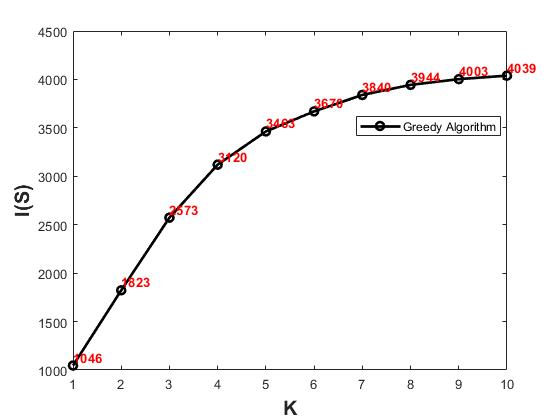
\includegraphics[width=0.5\textwidth]{fig/facebook.jpg}}   
   \subfloat [Pagerank Algorithm]{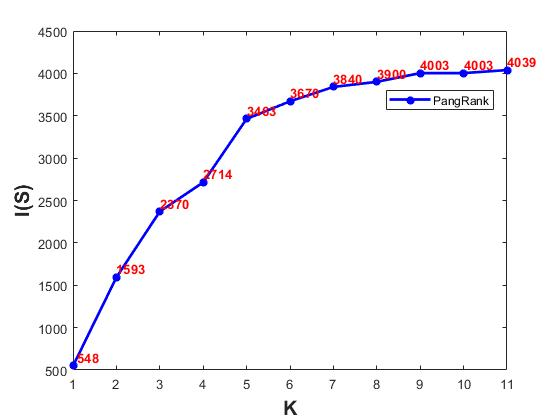
\includegraphics[width=0.5\textwidth]{fig/facebook_pagerank.jpg}}   
   \caption{The relation between the budget $K$ and {\itshape{influence}} $I(S)$ using our greedy algorithm and pagerank implementation. Note that beyond $K=10$ for the greedy algorithm (and $K=11$ for pagerank algorithm), the {\itshape{influence}} remains constant at value of 4039 since after this value the whole graph would be influenced/activated.  }
   \label{fig:inf}
\end{figure}


\paragraph{Part D:}
We used the pagerank algorithm in order to identify the VIP nodes and compute $S$. We started by constructing the \emph{column-stochastic matrix} $P$ from which pagerank algorithm can compute the score for all vertices. Since pagerank algorithm is designed for directed graph and our graph undirected, we considered edge undirected edge as two undirected edges. From that we can easily construct $P$ (as done in the first project). We then used pagerank to rank the different vertices. We tried two method to pick the VIP. The first one is simply to pick the vertices with highest pagerank score. This gave use almost the same vertices as the greedy algorithm gave. We were able to cover/influence the whole graph with $K=11$. Figure~\ref{fig:inf}(b). We superimposed both curved in Figure~\ref{fig:inf2}(a) to better visualize the performance of both. It is clear that the greedy algorithm outperform pagerank algorithm. However, with larger graphs, it is possible that pagerank might have better running time. 


The second method we used to identify the VIP from the pagerank scoring is a heuristic. The method starts by adding the highest rank vertex to $S$. It then proceed by adding the vertex that will return highest marginal gain. We do this by looping over the vertices in descending order with respect to their score. At each step in the loop, we compute the marginal gain of this vertex and compare it with the marginal gain of the next vertices that have less score than this vertex and pick the vertex the has the highest marginal gain and add it to $S$. This heuristic method is a little superior than the first method as shown in Figure~\ref{fig:inf2}(b). We still need $K=11$ in order to influence the whole graph. However, with $K=4$, the heuristic return larger number of influenced vertices. It could be possible with larger graphs, there could be multiple values of $K$ where heuristic method would be superior. Note that by design, the heuristic method could never give less influence that the first method; picking the vertices with highest score. 


\begin{figure}[!tbh]
\centering        
   \subfloat [Pagerank Algorithm]{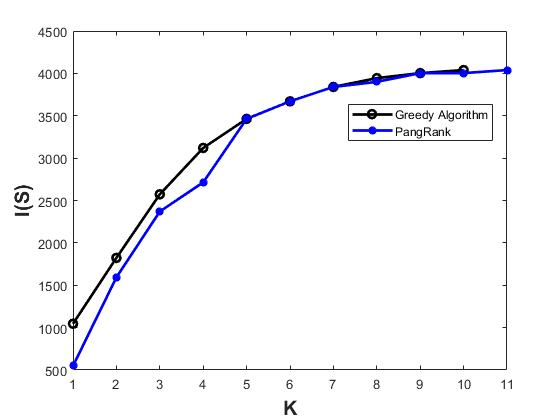
\includegraphics[width=0.5\textwidth]{fig/facebook_compare.jpg}}   
   \subfloat [Pagerank Algorithm]{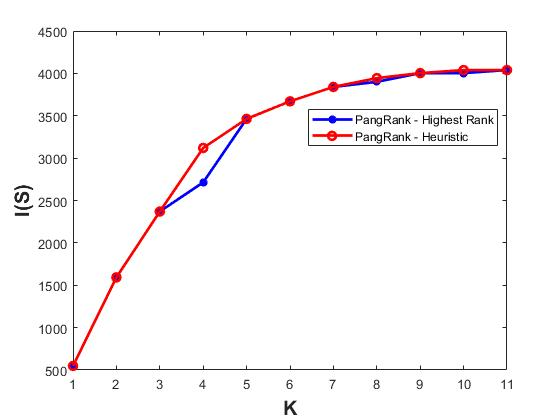
\includegraphics[width=0.5\textwidth]{fig/facebook_heuristic.jpg}}   
   
   
   \caption { Influence Maximization: (a) shows the comparison between the greedy algorithm performance and pagerank. (b) compares between two methods for picking the VIP vertices using pagerank algorithm; {\itshape{Highest Rank}} simply picks the $K$ vertices with highest rank,{\itshape{influence}} applies some heuristic in order to imporve the performance a little.}
   \label{fig:inf2}
\end{figure}
\paragraph{Other methods to measure influence:} One thing that our model(s) can't handle is the measuring the negative influence which can be added as negative weights over the edges. 